\documentclass[a4paper,11pt,fleqn,twoside,openright]{memoir} 	% Openright aabner kapitler paa hoejresider (openany begge)

%%%% PAKKER %%%%

% ¤¤ Oversaettelse og tegnsaetning ¤¤ %
\usepackage[utf8]{inputenc}					% Input-indkodning af tegnsaet (UTF8)
\usepackage[danish]{babel}					% Dokumentets sprog
\usepackage[T1]{fontenc}					% Output-indkodning af tegnsaet (T1)
\usepackage{ragged2e,anyfontsize}			% Justering af elementer
\usepackage{fixltx2e}						% Retter forskellige fejl i LaTeX-kernen
																			
% ¤¤ Figurer og tabeller (floats) ¤¤ %
\usepackage{graphicx} 						% Haandtering af eksterne billeder (JPG, PNG, PDF)
\usepackage{multirow}                		% Fletning af raekker og kolonner (\multicolumn og \multirow)
\usepackage{colortbl} 						% Farver i tabeller (fx \columncolor, \rowcolor og \cellcolor)
\usepackage[dvipsnames]{xcolor}				% Definer farver med \definecolor. Se mere: http://en.wikibooks.org/wiki/LaTeX/Colors
\usepackage{flafter}						% Soerger for at floats ikke optraeder i teksten foer deres reference
\let\newfloat\relax 						% Justering mellem float-pakken og memoir
\usepackage{float}							% Muliggoer eksakt placering af floats, f.eks. \begin{figure}[H]
%\usepackage{eso-pic}						% Tilfoej billedekommandoer paa hver side
%\usepackage{wrapfig}						% Indsaettelse af figurer omsvoebt af tekst. \begin{wrapfigure}{Placering}{Stoerrelse}
%\usepackage{multicol}         	        	% Muliggoer tekst i spalter
%\usepackage{rotating}						% Rotation af tekst med \begin{sideways}...\end{sideways}

% ¤¤ Matematik mm. ¤¤
\usepackage{amsmath,amssymb,stmaryrd} 		% Avancerede matematik-udvidelser
\usepackage{mathtools}						% Andre matematik- og tegnudvidelser
\usepackage{textcomp}                 		% Symbol-udvidelser (f.eks. promille-tegn med \textperthousand )
\usepackage{siunitx}						% Flot og konsistent praesentation af tal og enheder med \si{enhed} og \SI{tal}{enhed}
\sisetup{output-decimal-marker = {,}}		% Opsaetning af \SI (DE for komma som decimalseparator) 
\usepackage[version=3]{mhchem} 				% Kemi-pakke til flot og let notation af formler, f.eks. \ce{Fe2O3}
%\usepackage{rsphrase}						% Kemi-pakke til RS-saetninger, f.eks. \rsphrase{R1}

% ¤¤ Referencer og kilder ¤¤ %
\usepackage[danish]{varioref}				% Muliggoer bl.a. krydshenvisninger med sidetal (\vref)
\usepackage{natbib}							% Udvidelse med naturvidenskabelige citationsmodeller
%\usepackage{xr}							% Referencer til eksternt dokument med \externaldocument{<NAVN>}
%\usepackage{glossaries}					% Terminologi- eller symbolliste (se mere i Daleifs Latex-bog)

% ¤¤ Misc. ¤¤ %
\usepackage{listings}						% Placer kildekode i dokumentet med \begin{lstlisting}...\end{lstlisting}
\usepackage{lipsum}							% Dummy text \lipsum[..]
\usepackage[shortlabels]{enumitem}			% Muliggoer enkelt konfiguration af lister
\usepackage{pdfpages}						% Goer det muligt at inkludere pdf-dokumenter med kommandoen \includepdf[pages={x-y}]{fil.pdf}	
\pdfoptionpdfminorversion=6					% Muliggoer inkludering af pdf dokumenter, af version 1.6 og hoejere
\pretolerance=2500 							% Justering af afstand mellem ord (hoejt tal, mindre orddeling og mere luft mellem ord)

% Kommentarer og rettelser med \fxnote. Med 'final' i stedet for 'draft' udloeser hver note en error i den faerdige rapport.
\usepackage[footnote,draft,danish,silent,nomargin]{fixme}		


%%%% BRUGERDEFINEREDE INDSTILLINGER %%%%

% ¤¤ Marginer ¤¤ %
\setlrmarginsandblock{3.5cm}{2.5cm}{*}		% \setlrmarginsandblock{Indbinding}{Kant}{Ratio}
\setulmarginsandblock{2.5cm}{3.0cm}{*}		% \setulmarginsandblock{Top}{Bund}{Ratio}
\checkandfixthelayout 						% Oversaetter vaerdier til brug for andre pakker

%	¤¤ Afsnitsformatering ¤¤ %
\setlength{\parindent}{0mm}           		% Stoerrelse af indryk
\setlength{\parskip}{3mm}          			% Afstand mellem afsnit ved brug af double Enter
\linespread{1,1}							% Linie afstand

% ¤¤ Litteraturlisten ¤¤ %
\bibpunct[,]{[}{]}{;}{a}{,}{,} 				% Definerer de 6 parametre ved Harvard henvisning (bl.a. parantestype og seperatortegn)
\bibliographystyle{bibtex/harvard}			% Udseende af litteraturlisten.

% ¤¤ Indholdsfortegnelse ¤¤ %
\setsecnumdepth{subsection}		 			% Dybden af nummerede overkrifter (part/chapter/section/subsection)
\maxsecnumdepth{subsection}					% Dokumentklassens graense for nummereringsdybde
\settocdepth{subsection} 					% Dybden af indholdsfortegnelsen

% ¤¤ Lister ¤¤ %
\setlist{
  topsep=0pt,								% Vertikal afstand mellem tekst og listen
  itemsep=-1ex,								% Vertikal afstand mellem items
} 

% ¤¤ Visuelle referencer ¤¤ %
\usepackage[colorlinks]{hyperref}			% Danner klikbare referencer (hyperlinks) i dokumentet.
\hypersetup{colorlinks = true,				% Opsaetning af farvede hyperlinks (interne links, citeringer og URL)
    linkcolor = black,
    citecolor = black,
    urlcolor = black
}

% ¤¤ Opsaetning af figur- og tabeltekst ¤¤ %
\captionnamefont{\small\bfseries\itshape}	% Opsaetning af tekstdelen ('Figur' eller 'Tabel')
\captiontitlefont{\small}					% Opsaetning af nummerering
\captiondelim{. }							% Seperator mellem nummerering og figurtekst
\hangcaption								% Venstrejusterer flere-liniers figurtekst under hinanden
\captionwidth{\linewidth}					% Bredden af figurteksten
\setlength{\belowcaptionskip}{0pt}			% Afstand under figurteksten
		
% ¤¤ Opsaetning af listings ¤¤ %
\definecolor{commentGreen}{RGB}{34,139,24}
\definecolor{stringPurple}{RGB}{208,76,239}

\lstset{language=Matlab,					% Sprog
	basicstyle=\ttfamily\scriptsize,		% Opsaetning af teksten
	keywords={for,if,while,else,elseif,		% Noegleord at fremhaeve
			  end,break,return,case,
			  switch,function},
	keywordstyle=\color{blue},				% Opsaetning af noegleord
	commentstyle=\color{commentGreen},		% Opsaetning af kommentarer
	stringstyle=\color{stringPurple},		% Opsaetning af strenge
	showstringspaces=false,					% Mellemrum i strenge enten vist eller blanke
	numbers=left, numberstyle=\tiny,		% Linjenumre
	extendedchars=true, 					% Tillader specielle karakterer
	columns=flexible,						% Kolonnejustering
	breaklines, breakatwhitespace=true,		% Bryd lange linjer
}

% ¤¤ Navngivning ¤¤ %
\addto\captionsdanish{
	\renewcommand\appendixname{Appendiks}
	\renewcommand\contentsname{Indholdsfortegnelse}	
	\renewcommand\appendixpagename{Appendiks}
	\renewcommand\appendixtocname{Appendiks}
	\renewcommand\cftchaptername{\chaptername~}				% Skriver "Kapitel" foran kapitlerne i indholdsfortegnelsen
	\renewcommand\cftappendixname{\appendixname~}			% Skriver "Appendiks" foran appendiks i indholdsfortegnelsen
}

% ¤¤ Kapiteludssende ¤¤ %
\definecolor{numbercolor}{gray}{0.7}		% Definerer en farve til brug til kapiteludseende
\newif\ifchapternonum

\makechapterstyle{jenor}{					% Definerer kapiteludseende frem til ...
  \renewcommand\beforechapskip{0pt}
  \renewcommand\printchaptername{}
  \renewcommand\printchapternum{}
  \renewcommand\printchapternonum{\chapternonumtrue}
  \renewcommand\chaptitlefont{\fontfamily{pbk}\fontseries{db}\fontshape{n}\fontsize{25}{35}\selectfont\raggedleft}
  \renewcommand\chapnumfont{\fontfamily{pbk}\fontseries{m}\fontshape{n}\fontsize{1in}{0in}\selectfont\color{numbercolor}}
  \renewcommand\printchaptertitle[1]{%
    \noindent
    \ifchapternonum
    \begin{tabularx}{\textwidth}{X}
    {\let\\\newline\chaptitlefont ##1\par} 
    \end{tabularx}
    \par\vskip-2.5mm\hrule
    \else
    \begin{tabularx}{\textwidth}{Xl}
    {\parbox[b]{\linewidth}{\chaptitlefont ##1}} & \raisebox{-15pt}{\chapnumfont \thechapter}
    \end{tabularx}
    \par\vskip2mm\hrule
    \fi
  }
}											% ... her

\chapterstyle{jenor}						% Valg af kapiteludseende - Google 'memoir chapter styles' for alternativer

% ¤¤ Sidehoved/sidefod ¤¤ %

\makepagestyle{Uni}							% Definerer sidehoved og sidefod udseende frem til ...
\makepsmarks{Uni}{%
	\createmark{chapter}{left}{shownumber}{}{. \ }
	\createmark{section}{right}{shownumber}{}{. \ }
	\createplainmark{toc}{both}{\contentsname}
	\createplainmark{lof}{both}{\listfigurename}
	\createplainmark{lot}{both}{\listtablename}
	\createplainmark{bib}{both}{\bibname}
	\createplainmark{index}{both}{\indexname}
	\createplainmark{glossary}{both}{\glossaryname}
}
\nouppercaseheads											% Ingen Caps oenskes

\makeevenhead{Uni}{Gruppe B131}{}{\leftmark}				% Lige siders sidehoved (\makeevenhead{Navn}{Venstre}{Center}{Hoejre})
\makeoddhead{Uni}{\rightmark}{}{Dit Universitet}			% Ulige siders sidehoved (\makeoddhead{Navn}{Venstre}{Center}{Hoejre})
\makeevenfoot{Uni}{\thepage}{}{}							% Lige siders sidefod (\makeevenfoot{Navn}{Venstre}{Center}{Hoejre})
\makeoddfoot{Uni}{}{}{\thepage}								% Ulige siders sidefod (\makeoddfoot{Navn}{Venstre}{Center}{Hoejre})
\makeheadrule{Uni}{\textwidth}{0.5pt}						% Tilfoejer en streg under sidehovedets indhold
\makefootrule{Uni}{\textwidth}{0.5pt}{1mm}					% Tilfoejer en streg under sidefodens indhold

\copypagestyle{Unichap}{Uni}								% Sidehoved defineres som blank på kapitelsider
\makeoddhead{Unichap}{}{}{}
\makeevenhead{Unichap}{}{}{}
\makeheadrule{Unichap}{\textwidth}{0pt}
\aliaspagestyle{chapter}{Unichap}							% Den ny style vaelges til at gaelde for chapters
															% ... her
															
\pagestyle{Uni}												% Valg af sidehoved og sidefod (benyt "plain" for ingen sidehoved/fod)


%%%% EGNE KOMMANDOER %%%%

% ¤¤ Billede hack ¤¤ %										% Indsaet figurer nemt med \figur{Stoerrelse}{Fil}{Figurtekst}{Label}
\newcommand{\figur}[4]{
		\begin{figure}[H] \centering
			\includegraphics[width=#1\textwidth]{billeder/#2}
			\caption{#3}
			\label{#4}
		\end{figure} 
}

% ¤¤ Specielle tegn ¤¤ %
\newcommand{\decC}{^{\circ}\text{C}}
\newcommand{\dec}{^{\circ}}
\newcommand{\m}{\cdot}


%%%% ORDDELING %%%%

\hyphenation{In-te-res-se e-le-ment}
\begin{document}
Induktiv kopling:
\begin{itemize}
\item Elektriske felter
\begin{itemize}
\item Gauss's lov
\end{itemize}
\end{itemize}

Inden vi begynder at beregne den strøm, der bliver induseret mellem den trådløse oplader og det elektriske apparat, så skal vi have bedre kendskab til elektriske felter. Til dette skal vi se nærmere på Gauss's lov, der beskriver elektrisk flux gennem forholdet mellem det elektriske felt og det areal, det passerer ved en lukket overflade.

Først kan vi definere formlen for flux, som angiver det elektriske felt ganget med arealet, det løber igennem: $\Phi = E * A$. Da indfaldsvinklen for det elektriske felt også har betydning, så ser vi $\vec{E} \bullet \vec{A}$ i stedet for, hvilket også kan opskrives som $\Phi = E * A * cos(\theta)$. (Se figur X)
%Figur af elektrisk felt vinkelret og vinklet på overflade

\begin{figure}[H]
\centering
%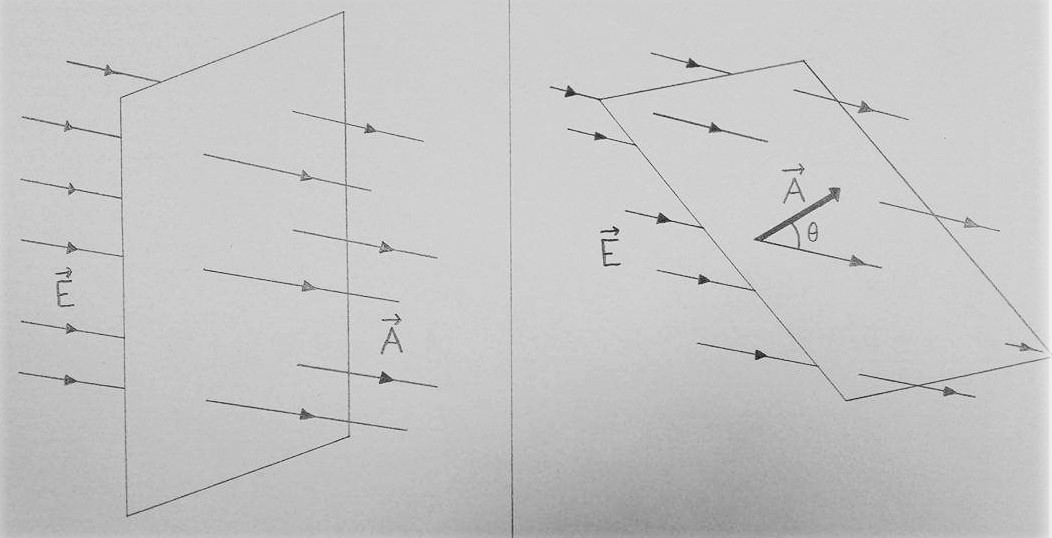
\includegraphics[scale=0.5]{vinkelflux}
\caption{Figur X}
\end{figure}

Gauss's lov angiver ikke kun den elektriske flux, men den kan benyttes til at beregne den flux, der forløber over et bestemt areal. Derved skal vi integrere i forhold til overfladen, samt at vektor A skal ganges med en faktor d, så vi får $\Phi = \int \vec{E} \bullet d \vec{A}$, som igen kan skrives som $\Phi = \int E * dA * cos(\theta)$. Herefter tager Gauss relation til det cirkulære felt omkring en positiv ladning. A bliver i denne sammenhæng formlen for en kugles overflade $4 \pi r^2$, mens integralet ophæves, da vi nu omtaler hele overfladen igen. Herfra får vi: $\Phi = E * 4 \pi r^2$

Det elektriske felt E er også angivet til at være $\frac{kq}{r^2}$. Ud fra dette får vi den elektriske flux til: $\Phi = \frac{kq}{r^2} * 4 \pi r^2 = 4 \pi k q$. k er derudover defineret som $\frac{1}{4 \pi \epsilon_0}$, hvilket vi kan indsætte i forrige formel, hvorved vi får: $\frac{4 \pi q}{4 \pi \epsilon_0} = \frac{q}{\epsilon_0}$.

q angiver den omkransede ladning for en lukket overflade. Derved kan vi opskrive Gauss's lov til følgende:

\centerline{$\oint \vec{E} \bullet d \vec{A} = \frac{q}{\epsilon_0}$}

\begin{itemize}
\item Elektromagnetisme
\begin{itemize}
\item Ampère's lov
\end{itemize}
\end{itemize}
Ampère's lov beskriver relationen mellem magnetiske feltstyrker og størrelsen af en jævn strøn gennem en ledning givet over længden l. Ampère tager udgangspunkt i, hvis man befinder sig ved ledningens center og følger magnetfeltet, som omkredser ledningen. Her er magnetfeltets styrke defineret ved vektoren $\vec{B}$, og et definerede linjestykke af magnetfeltets længde angives som $\vec{dl}$. For at beregne den jævne strøm gennem ledningen, skal vi tage integralet af de to vektorer prikket sammen. Herved beskrives Ampére's lov:

\centerline{$\oint \vec{B} \bullet \vec{dl} = \mu_0 I$}

Vektor $\vec{B}$ er angivet ved $\frac{\mu_0 I}{2 \pi r}$, da vi arbejder med et cirkelformet magnetfelt. Derudover er det lukkede integrale af $\vec{dl}$ den totale længde af cirkelperiferien angivet ved $2 \pi r$. Produktet mellem disse vil dermed blive $\mu_0 I$, som vi ser på højre side af Ampére's lov.


\begin{itemize}
\item Faraday's lov
\end{itemize}
En af de begreber, som elektromagnetisme beskriver, er induktion af spænding ved hjælp af magnetisme. Før vi ser på Faraday's lov, skal vi kende begrebet magnetisk flux. Magnetisk flux ligner til delt elektrisk flux, som beskrevet tidligere. Her tager man integralet over det magnetiske felt prikket med et bestemt overfladeareal: $\Phi_B = \int \vec{B} \bullet \vec{dA}$

En induseret strøm opstår ikke fra den magnetiske flux alene, men ved en ændring i den magnetiske flux. Dette betyde, at der bliver induseret spænding, hvis der sker en ændring af magnetfeltets styrke, den påvirkede overflades størrelse eller vinklen for, hvordan det magnetiske felt går gennem den pågældende overflade.

Faraday benytter den magnetiske flux til at beskrive den inducerede spænding ved:

\centerline{$\varepsilon = -1 * \frac{d \Phi_B}{dt}$}

Ændringen af den magnetiske flux optræder ofte modsat af den inducerede spænding, så derfor ganger Faraday en faktor -1 på det differentierede udtryk af den magnetiske flux. Den magnetiske flux kan også beskrives som $\vec{B} \bullet \vec{A}$ eller $B * A * cos(\theta)$.
\begin{itemize}
\item Maxwell's ligninger (Forbindelse mellem Faraday og Ampère)
\end{itemize}
Ved trådløs opladning arbejder man med at omdanne elektrisk flux til magnetisk flux gennem spolen ved transmitteren, hvorefter den magnetiske flux igen skal omdannes til en elektrisk flux ved modtageren. For at beskrive hvordan elektriske felter omdannes til magnetisk flux, så skal vi se nærmere på Ampére's lov. Herefter kan overgangen fra magnetfelt til elektrisk flux beskrives gennem Faraday's lov. Til slut kan vi se på Maxwell's ligninger, som bygger videre på Ampère's og Faraday's love, hvorved vi kan skabe en sammenhæng.

Maxwell indså, at der måtte foretages modifikationer for Ampére's lov, hvis der skulle kunne skabes symmetri med Faraday's lov. Ved Maxwell's ligninger er Faraday's lov opgivet som det lukkede linjeintegrale af det magnetiske felt, som er lig det negative differentiale af den magnetiske flux i forhold til tid: $\oint \vec{E} \bullet \vec{dl} = -1 * \frac{d \Phi_B}{dt}$.

Herefter kan vi kaste et blik på Maxwell's modificerede udgave af Ampère's lov. Maxwell har her udbygget formlen, så der skabes en symmetri med Faraday's lov. Derved bliver Ampère's lov omskrevet til, at det lukkede linjeintegrale af det magnetiske felt er lig den elektriske spænding lagt sammen med differentialet af den elektriske flux i forhold til tiden, hvorpå der er ganget en faktor bestående af produktet mellem permeabilitetskonstanten og permittivitetskonstanten: $\oint \vec{B} \bullet \vec{dl} = \mu_0 * I + \mu_0 \epsilon_0 * \frac{d \Phi_E}{dt}$.

Grunden til, at Maxwell udbygger Ampère's lov, er, at loven kun er gældende for, at en stabil strøm er med til at danne en magnetisk flux. For at skabe symmetri med Faraday, udformede Maxwell sin teori om, at elektrisk flux også er gældende for at danne magnetisk flux ved en ustabil strøm. Derved er udtrykket $\mu_0 \epsilon_0 * \frac{d \Phi_E}{dt}$ tilføjet til det oprindelige udtryk.
\end{document}